\chapter{Background}\label{Background}

This chapter offers an overview of the technology and concepts needed to understand the context and relevance of the work within the broader world. The review is conducted predominately through a networking, security and privacy perspective to best highlight the aspects pertinent to the distributed deployment of ECH. This chapter also represents the bulk of the effort put into investigating and studying the functioning of ECH while identifying and experimenting with different deployment models.

This chapter<contents and why "we see how trans and the domain name interacts with ech" "inspect the functioning of ech" "">
This chapter<contents and why "we see how trans and the domain name interacts with ech" "inspect the functioning of ech" "">
This chapter<contents and why "we see how trans and the domain name interacts with ech" "inspect the functioning of ech" "">








\section{Transport Layer Security}

Transport Layer Security (TLS) is a cryptographic protocol proposed by the Internet Engineering Task Force (IETF) which enables secure network communication over public networks. Applications and services can establish an encrypted communication channel to transmit private information such that confidentiality, integrity and authenticity of the data can be ensured. TLS is commonly used to protect Internet traffic, having seen widespread adoption and several revisions since its original inception in 1999, superseding the Secure Sockets Layer (SSL) specification previously defined by Netscape Communications from 1994~\cite{chan2018monitoring, LE-HTTPS, rfc2246}.

TLS is designed to operate on top of a reliable transmission protocol between a client and server, such as the Transmission Control Protocol (TCP) when used over the Internet. In order to prevent eavesdropping, tampering and message forgery, TLS includes a number of security features based on a number of cryptographic mechanisms:

\begin{description}
	\item[Confidentiality] All service and application data exchanged between the client and server is encrypted as to make it indecipherable to any intermediate party which might be intercepting their communication.
	\item[Data integrity] In a similar manner, cryptographic properties are used to guarantee all transferred data cannot be modified during transmission.
	\item[Authentication] TLS provides the ability for both participants to verify the identity of the other, ensuring privileged communication is only performed with the intended recipient.
\end{description}

TLS 1.3 is the latest defined standard for the protocol, having been published in August 2018 and contributing to the deprecation of TLS 1.0 and TLS 1.1 in March 2021~\cite{rfc8446, rfc8996}. <It introduces many major changes to TLS 1.2 which enables numerous new <encryption of handshake>>

\subsection{Digital Certificates}

TLS uses digital certificates to make assertions on the identity of entities within the network. These certificates contain <> which enables , provided a number of <steps>

These certificates are exchanged during the establishment of secure communication between the client and server to . Their <functioning> is based on a number

<public key, trust>

\begin{figure}[ht]
\centerline{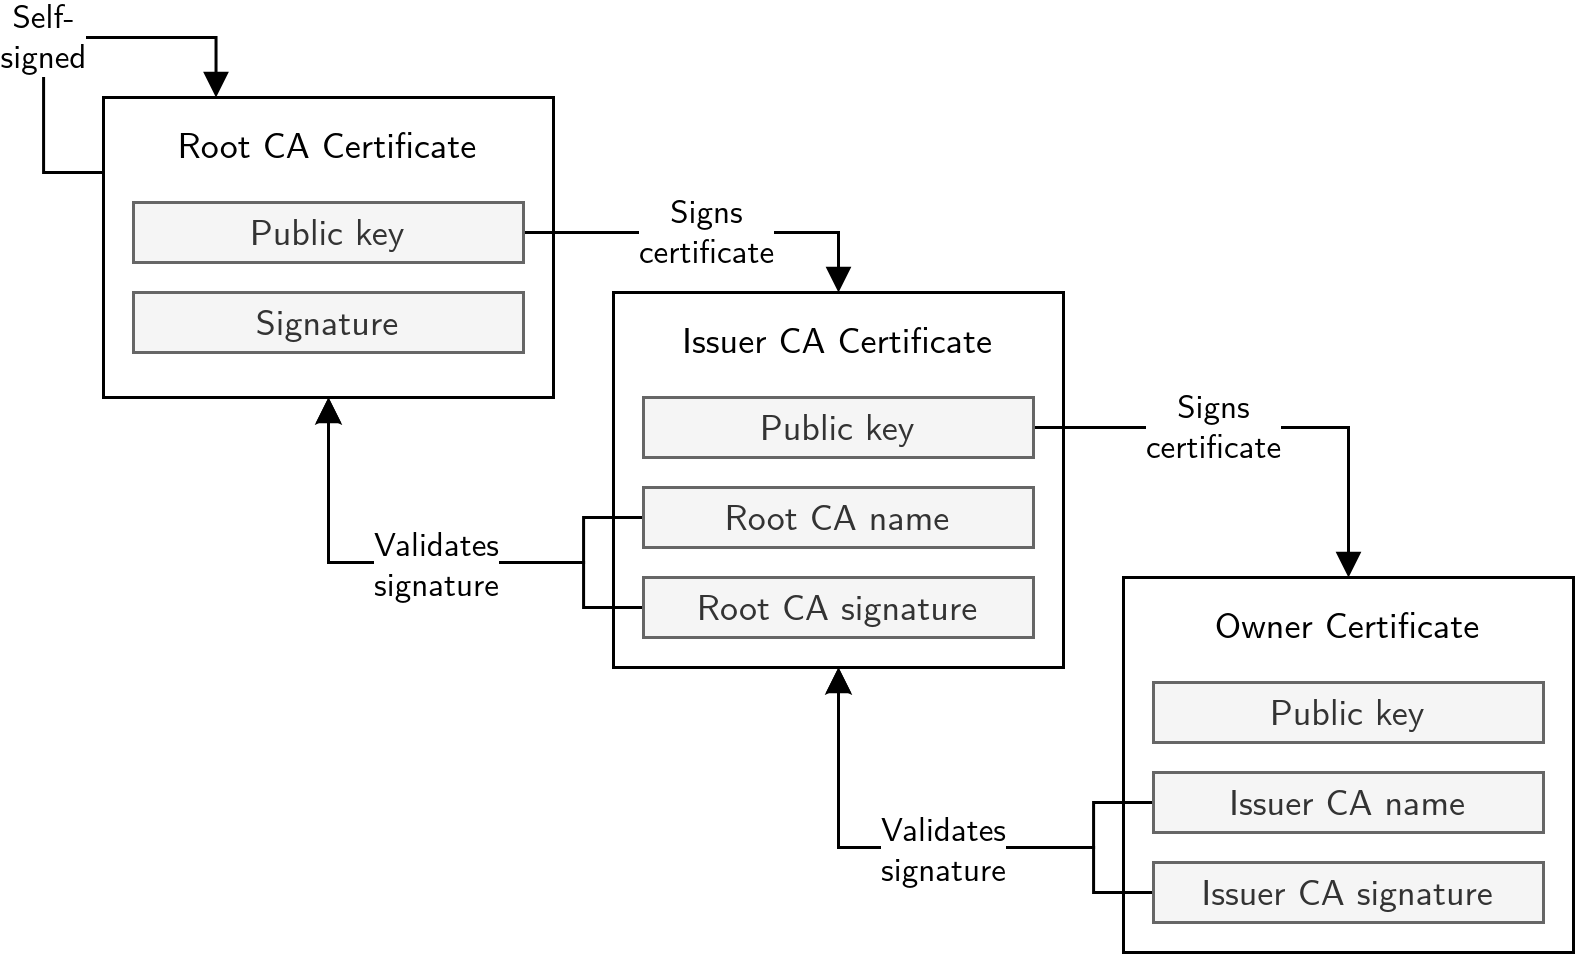
\includegraphics[width=160mm]{images/tls-chain.png}}
\caption[TLS certificate chain of trust]{<>}
\label{tls_chain_figure}
\end{figure}

\subsection{Handshake}

\begin{figure}[ht]
\centerline{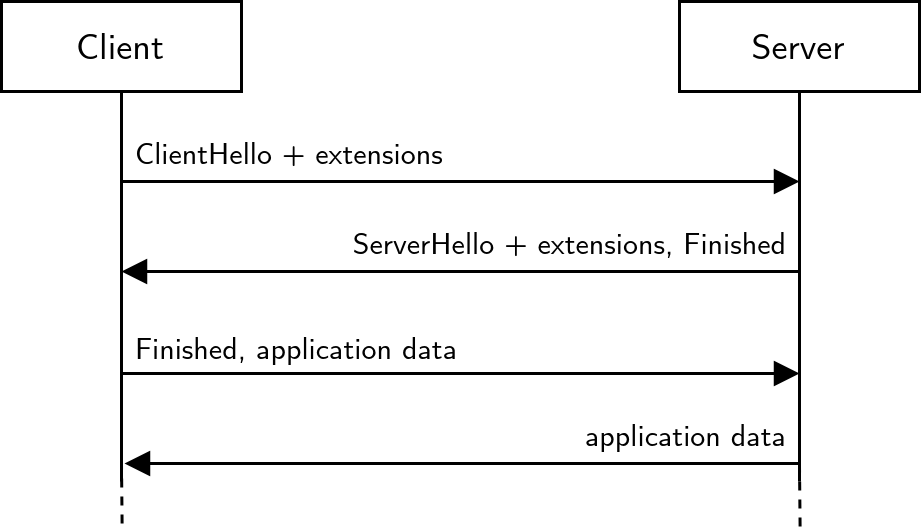
\includegraphics[width=160mm]{images/tls-handshake.png}}
\caption[Basic TLS 1.3 handshake]{<>}
\label{tls_handshake_figure}
\end{figure}

\begin{description}
	\item[ClientHello] <>
	\item[ServerHello] <>
\end{description}

<application data>

\subsection{Extensions}

<is>
<greasing>








\section{The Domain Name System}

<is>
<purpose>

\subsection{Name Resolution Process}

<>

\begin{figure}[ht]
\centerline{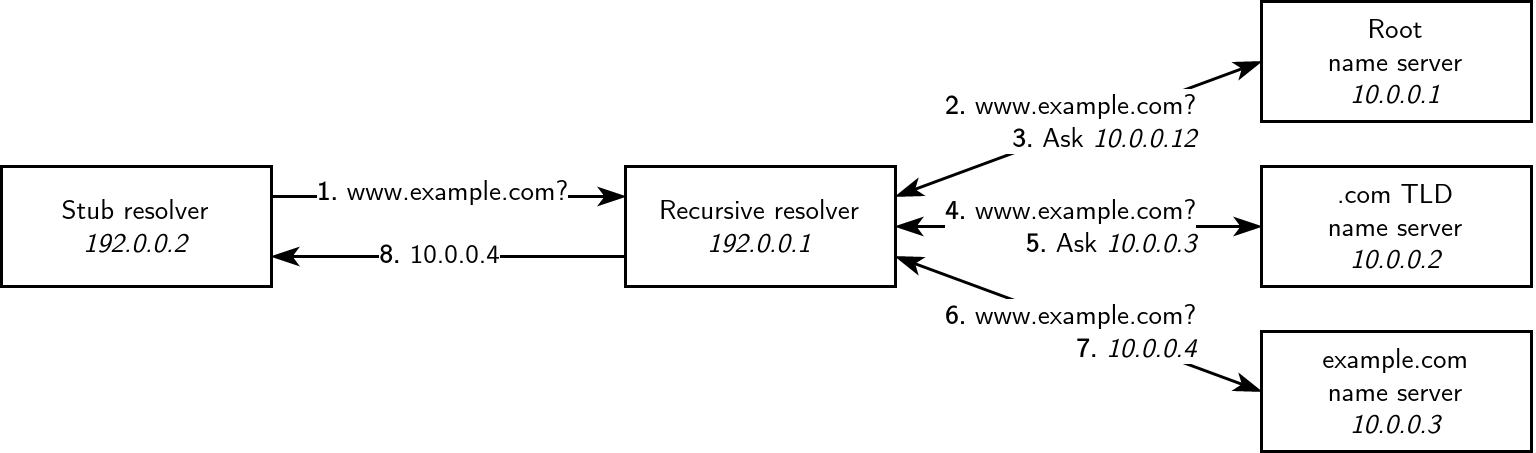
\includegraphics[width=160mm]{images/dns-resolve.png}}
\caption[Example DNS name resolution process]{<>}
\label{dns_resolve_figure}
\end{figure}

\subsection{DNS Over HTTPS}

\blindtext

\subsection{The HTTPS Resource Record}

\blindtext








\section{Encrypted Client Hello}

\blindtext

\subsection{Hybrid Public Key Encryption}

\blindtext

\subsection{Split Mode Deployment}

\blindtext

\begin{figure}[ht]
\centerline{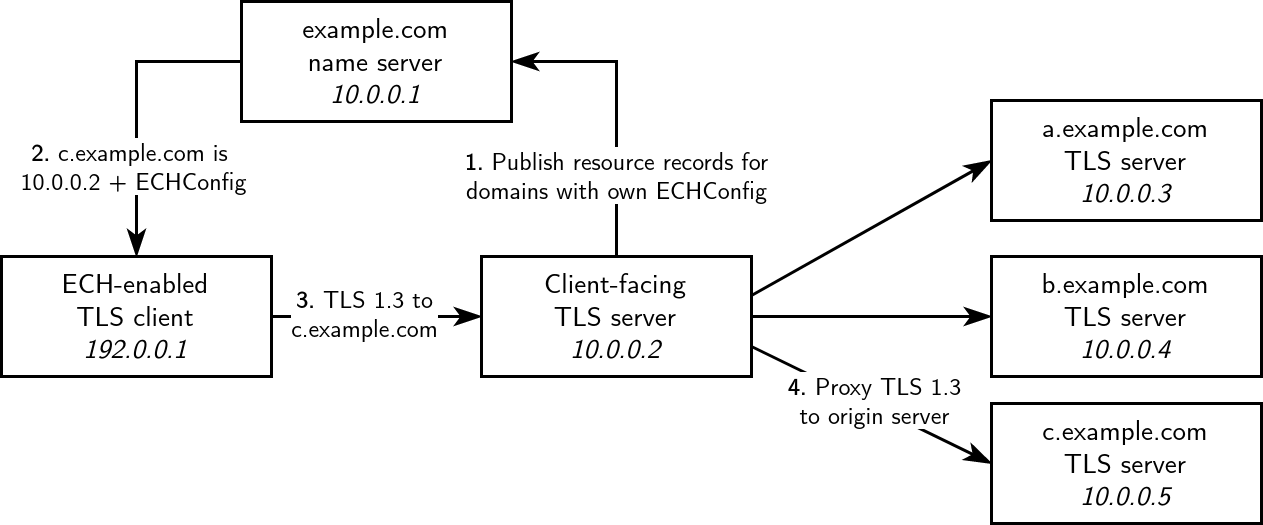
\includegraphics[width=160mm]{images/ech-split-mode.png}}
\caption[Example ECH Split Mode deployment]{<>}
\label{ech_split_mode_figure}
\end{figure}








\section{Traffic Analysis}

\blindtext

\subsection{Correlation Attacks}

\blindtext

\subsection{Traffic Padding}

\blindtext








\section{Summary}

\blindtext
